\documentclass[runningheads,a4paper]{llncs}

\usepackage{amssymb}
\setcounter{tocdepth}{3}
\usepackage{graphicx}
\usepackage[inline]{trackchanges}

\usepackage{url}
\urldef{\mails}\path|{claas.wilke, michael.thiele, c.wende}@inf.tu-dresden.de|
\newcommand{\keywords}[1]{\par\addvspace\baselineskip
\noindent\keywordname\enspace\ignorespaces#1}

% For german character �,�,�,�
\usepackage[latin1]{inputenc}

\begin{document}

\mainmatter  % start of an individual contribution

% first the title is needed

\title{Defining and Interpreting OCL Constraints on Arbitrary Models and Model
Instances \note{the term model instance is not very common and easy to distinguish from
model. What do you think of model implementations?}}

% a short form should be given in case it is too long for the running head
\titlerunning{Defining and Interpreting OCL on Arbitrary Models and Model Instances}

% the name(s) of the author(s) follow(s) next
%
% NB: Chinese authors should write their first names(s) in front of
% their surnames. This ensures that the names appear correctly in
% the running heads and the author index.
%
\author{Claas Wilke\and Michael Thiele\and Christian Wende\\
\mails}
%
\authorrunning{Defining and Interpreting OCL on Arbitrary Models and Model Instances}
% (feature abused for this document to repeat the title also on left hand pages)

% the affiliations are given next; don't give your e-mail address
% unless you accept that it will be published
\institute{Technische Universit�t Dresden\\
Department of Computer Science\\
Institute for Software and Multimedia Technology\\
Software Technology Group
%\url{http://www.st.inf.tu-dresden.de}
}

%
% NB: a more complex sample for affiliations and the mapping to the
% corresponding authors can be found in the file "llncs.dem"
% (search for the string "\mainmatter" where a contribution starts).
% "llncs.dem" accompanies the document class "llncs.cls".
%

\toctitle{Lecture Notes in Computer Science}
\tocauthor{Authors' Instructions}
\maketitle

\note{do we use british or american english?}
\begin{abstract}
In recent years the Object Constraint Language (OCL) has become a popular 
constraint language that is used \change{on top of}{in combination with}
multiple modeling languages such as UML, EMF Ecore and various domain specific 
languages. \remove{OCL is only loosely coupled to these modeling languages, }It
is rather common to reuse the same OCL parsers for multiple different modeling 
languages. 
\change{While OCL-annotated models are implemented and instantiated in various
implementation languages, dynamic OCL semantics as required for OCL constraint 
interpretation is typically bound to a specific implementation language.} 
In this paper, we propose an architecture for an OCL tool that
\change{encapsulates}{hides} meta-models, models and model
\change{instances in specific implementation languages} behind well-defined
interfaces. We present an OCL interpreter that can interpret OCL constraints 
on various different model \change{instantiations}{implementations} and
\change{provides}{, thus, enables} reuse of the same dynamic OCL semantics
implementation for all these \change{instantiation types}{implementation types}.
The architecture is evaluated \change{by presenting}{in} three case studies
defining and interpreting OCL constraints on multiple models and model
\change{instances}.

\keywords{OCL, MDSD, Modeling, Constraint Interpretation.}
\end{abstract}

  \chapter{Getting started with Dresden OCL}
\label{chapter:introduction}

\begin{flushright}
\textit{Chapter written by Claas Wilke and Michael Thiele}
\end{flushright}

This chapter generally introduces into \keyword{Dresden OCL}. Dresden OCL is
based on a \keyword{Pivot Model} developed by Matthias 
Br�uer~\cite{GB:Braeuer} which is shortly explained in 
Chapter~\ref{chapter:architecture}. Further information about Dresden OCL is 
available at the project's website~\cite{WWW:toolkit}.

This chapter explains the installation of Dresden OCL and how to load a 
model, an instance of such a model, and \acs{OCL} constraints defined on such a 
model into Dresden OCL. Besides the Eclipse distribution, Dresden OCL can 
also be used as a stand-alone Java library. If you plan to use the stand-alone 
distribution you can skip this chapter and continue with 
Chapter~\ref{chapter:standalone}. However, this chapter explains the basic 
concepts of Dresden OCL. Although you cannot use the shown GUI wizards and 
browsers when using the stand-alone version, this chapter can be helpful to 
understand the terms used in and the mechanisms provided by Dresden OCL.
  


\section{How to Install Dresden OCL}
	
The following different possibilities exist to install Dresden OCL within
Eclipse.

\begin{enumerate}
	\item You may install Dresden OCL using the \emph{Eclipse Marketplace
	  Client}.
	\item You may install Dresden using the update site available
	  at~\cite{WWW:toolkitUpdatesite},
	\item You may checkout and run the source code distribution from the \acs{SVN}
	  available at~\cite{WWW:toolkitSVN}.
\end{enumerate}

This section will explain all three possibilities.
	

\subsection{Installing Dresden OCL using the Eclipse Marketplace Client}

Since Eclipse 3.6, the new Eclipse Marketplace Client allows easy installation
of Eclipse-based tools such as Dresden OCL.

To install Dresden OCL via the Eclipse Marketplace Client, select the menu
option \emph{Help -> Eclipse Marketplace\ldots}. Probably you have to select a
marketplace catalog afterwards. If so, select the \emph{Eclipse Marketplace}
catalog and proceed.

Type \texttt{Dresden OCL} into the search text field and press the return key.
Select Dresden OCL from the search results and click the \emph{Install} button
(cf. Fig.~\ref{pic:intro:marketplace01}). Afterwards, click through the
installation dialog and Dresden OCL will be installed. Finally you have to 
restart your Eclipse distribution to complete the installation.

\begin{figure}[!b]
	\centering
	\includegraphics[width=0.8\linewidth]{figures/introduction/marketplace01}
	\caption{Installing Dresden OCL using the Marketplace Client.}
	\label{pic:intro:marketplace01}
\end{figure}


\subsection{Installing Dresden OCL using the Eclipse Update Site}
	
To install Dresden OCL via the \keyword{Eclipse Update Site}, you have to
start an Eclipse instance and select the menu option \eclipse{Help ->
Install New Software\ldots}

Enter the path \url{http://www.dresden-ocl.org/update/site.xml} and
click the \eclipse{Add...} button (cf. Fig.~\ref{pic:intro:updateSite01}). 
In the new opened window you can additionaly enter a name for the update site 
(cf. Fig.~\ref{pic:intro:updateSite02}).

\begin{figure}[!b]
	\centering
	\includegraphics[width=0.8\linewidth]{figures/introduction/updateSite01}
	\caption{Adding an Eclipse Update Site (Step 1).}
	\label{pic:intro:updateSite01}

  \vspace{2.0em}
  
	\centering
	\includegraphics[width=0.6\linewidth]{figures/introduction/updateSite02}
	\caption{Adding an Eclipse Update Site (Step 2).}
	\label{pic:intro:updateSite02}
\end{figure}

Now you can select the features of Dresden OCL which you want to install. 
Select them and click the \eclipse{Next >} button (cf. 
Fig.~\ref{pic:intro:updateSite03}). An overview on all features of 
Dresden OCL can be found in Table~\ref{tab:plugins} in the appendix of 
this manual. Follow the wizard and agree with the user license. Then Dresden OCL
will be installed. Afterwards, you should restart your Eclipse application to 
finish the installation.

\begin{figure}[t]
	\centering
	\includegraphics[width=1.0\linewidth]{figures/introduction/updateSite03}
	\caption{Selecting features of Dresden OCL.}
	\label{pic:intro:updateSite03}
\end{figure}
	
	
\subsection{Importing Dresden OCL from the SVN}

To use Dresden OCL by checking out the source code from the \acs{SVN} you
need to install an \acs{SVN} client. In the following the 
\keyword{Eclipse Subversive} plug-in is used.

After installing Eclipse Subversive, a new \keyword{Eclispe Perspective} 
providing access to \acs{SVN} should exist. The perspective can be opened via 
the menu \eclipse{Window > Open Perpective > Other... > SVN Repository
Exploring}. In the view \eclipse{\acs{SVN} Repositories} you can add a new 
repository using the \acs{URL} 
\url{http://svn-st.inf.tu-dresden.de/svn/dresdenocl/} (cf. 
Fig.~\ref{pic:intro:svn01}).

\begin{figure}[!b]
	\centering
	\includegraphics[width=0.4\linewidth]{figures/introduction/svn01}
	\caption{Adding an SVN repository.}
	\label{pic:intro:svn01}
\end{figure}

After clicking the \eclipse{Finish} button, the \acs{SVN} repository root should 
be visible in the \eclipse{\acs{SVN} Repositories} view. To checkout the
plug-ins, you have to select them in the repository directory 
\reference{trunk/ocl20\-for\-Eclipse/eclipse} and use the \eclipse{Checkout...} 
function in the context menu (cf. Fig.~\ref{pic:intro:svn02}).
	
\begin{figure}[!t]
	\centering
	\includegraphics[width=0.4\linewidth]{figures/introduction/svn02}
	\caption{Checkout of Dresden OCL's plug-in projects.}
	\label{pic:intro:svn02}
\end{figure}


\subsection{Which Plug-ins do you need at least?}

Often people wonder which plug-ins of Dresden OCL they require for a
minimum installation. The answer to this question depends on the things you 
plan to do with Dresden OCL. Table~\ref{tab:plugins} in the appendix of 
this manual shows a list of the currently existing plug-ins of
Dresden OCL, that are related to different features. You should install 
at least the \keyword{Core} feature, at least one metamodel of the 
\keyword{Metamodels} feature, and the complete \keyword{Parser} feature. The 
\keyword{Interpreter}, the \keyword{OCL22Java} and the
\keyword{OCL2SQL} features are only required if you want to interpret
constraints or to generate code from constraints, respectively. If you import or interpret model instances, you need to install 
the \keyword{Model Instances} feature as well. The examples of the 
\keyword{Example} feature are only required to run the examples provided in 
this manual. We recommend to install all provided features.
		

\subsection{Building the OCL2 Parser}
The new Dresden OCL parser/editor is partially written in Scala. In order
to build the sources of the parser without having to have the \reference{Scala
IDE} installed, Dresden OCL comes with various \keyword{Ant} scripts that
compile the Scala code to byte code.

After a checkout, the build script should be called automatically. Be aware that
the compilation might take a while to finish. If other projects that depend on
the parser like the facade still do not compile correctly, try to perform a 
\keyword{refresh} on the plug-ins that contain Scala code.

If the \keyword{Ant} script is not invoked automatically, you can call it either
be cleaning the
\reference{tudresden\linebreak[0].ocl\-20\linebreak[0].pivot.language.ocl.staticsemantics}
plug-in or by running the \keyword{Ant} task \reference{clean all} of the same plug-in.

You have to run the \keyword{ANT} scripts in the same 
\keyword{JRE} as Eclipse. Figures~\ref{pic:intro:parserbuild01} 
and~\ref{pic:intro:parserbuild02} show how to achieve this. If an error like 
``Unable to find javac compiler.'' occurs, you might be trying to run the
\keyword{Ant} script with a \keyword{\acl{JRE}} instead of a \keyword{\acs{JDK}}
(For errors like this one) use the \eclipse{Installed JREs...} button in the
same window to select a \acs{JDK} instead.

If you want to make changes to the static semantics evaluation of the parser you
should consider installing the \emph{Scala IDE} from 
\url{http://www.scala-lang.org/scala-eclipse-plugin}. Be aware that the Scala
code is version 2.7.7 which is not compatible with Scala 2.8 and therefore you
cannot use the current \emph{Scala IDE} which supports only Scala 2.8. 

In order to use the Scala compiler of the IDE, you have to go to the
\eclipse{Properties} of each Scala plug-in, select the tab \eclipse{Builders},
check the \eclipse{Scala Builder} and possibly uncheck the \keyword{Ant} script
for building.

\begin{figure}[p]
	\centering
	\includegraphics[width=0.8\linewidth]{figures/introduction/parserbuild01}
	\caption{Executing the OCL2 Parser build script.}
	\label{pic:intro:parserbuild01}

  \vspace{4.0em}

	\centering
	\includegraphics[width=0.8\linewidth]{figures/introduction/parserbuild02}
	\caption{Settings of the JRE for the Ant build script.}
	\label{pic:intro:parserbuild02}

  \vspace{4.0em}

	\centering
	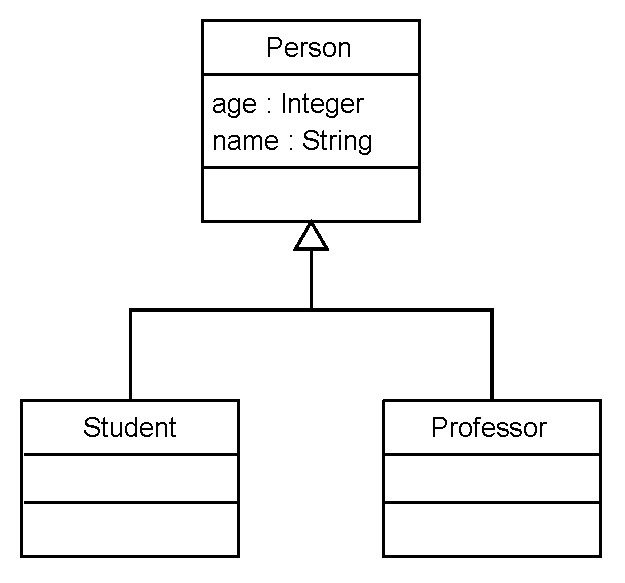
\includegraphics[width=0.5\linewidth]{figures/examples/simple01}
	\caption{A class diagram describing the Simple Example model.}
	\label{pic:examples:simple01}
\end{figure}


\section{Loading Models, Model Instances and Constraints}

If you installed the Dresden OCL using the market place client or update site,
you can execute the toolkit within your Eclipse distribution. If you imported
the Toolkit as source code plug-ins into an Eclipse workspace, you have to start a 
new Eclipse instance. You can start a new instance via the menu \eclipse{Run >
Run As > Eclipse Application}. If the menu \eclipse{Eclipse Application} is not 
available or disabled you need to select one of the plug-ins of the toolkit in
the \eclipse{Package Explorer} first.


\subsection{The Simple Example}
\label{intro:simpleExample}

The use of Dresden OCL is explained using the \keyword{Simple Example} 
which is located in the plug-in 
\reference{tudresden.ocl20.pivot.examples.\linebreak[0]simple}. 
Figure~\ref{pic:examples:simple01} shows a class diagram of the Simple Example.

Dresden OCL provides more examples than the Simple Example. The different 
examples use different metamodels which is possible with the \textit{Pivot
Model} architecture of the Toolkit. An overview on all examples provided 
with Dresden OCL is listed in Table~\ref{tab:examples} in the appendix of
this manual. The Simple Example can be used with two different metamodels. 
These are \keyword{\acs{UML}~2} (based on \keyword{\acs{Eclipse MDT} 
\acs{UML}}) and \keyword{Java}.


\subsection{Dresden OCL Perspective}

Dresden OCL provides its own perspective within Eclipse that contains all views
and editors provided with Dresden OCL. To ease the work with Dresden OCL, you
should now switch to the Dresden OCL perspective. Select the menu option
\eclipse{Window -> Open Perspective -> Other \ldots} and select the perspective
\eclipse{Dresden OCL} (cf. Fig.~\ref{pic:introduction:perspective}).
	
\begin{figure}[!t]
	\centering
	\includegraphics[width=1.0\linewidth]{figures/introduction/perspective}
	\caption{The Dresden OCL Perspective.}
	\label{pic:introduction:perspective}
\end{figure}

On the left hand side the perspective contains the \eclipse{Project Explorer} of
Eclipse to manage different projects. The right hand side contains the
\eclipse{Outline View} for opened \acs{OCL} files. Below, the \eclipse{Model
Browser} and \eclipse{Model Instance Browser} of Dresden OCL allow to explore models and
instances imported into Dresden OCL. At the bottom of the perspective the
\eclipse{OCL Intepreter} is located. The center of the perspective contains the
\eclipse{OCL Editor} of Dresden OCL that allows to edit and parse \acs{OCL}
files for an opened model. How to use the tools provided with Dresden OCL is explained in
the following.


\subsection{Loading a Model}
	
For this tutorial you first have to load a model into Dresden OCL. To ease the
use of the Simple Example project, this project should be imported into the  
\keyword{Workspace} first. Select the menu option \emph{File -> New ->
Other} and select the option \emph{Dresden OCL Examples -> Simple Example}
within the new opened window (cf. Fig~\ref{pic:intro:importexample01}). Click
the \emph{Finish} button to import the project into your workspace. Afterwards, the workspace should contain the Simple
Example project as shown in Figure~\ref{pic:introduction:perspective}, left hand
side.

\begin{figure}[!t]
	\centering
	\includegraphics[width=0.8\linewidth]{figures/introduction/importexample01}
	\caption{Importing the Simple Example project.}
	\label{pic:intro:importexample01}
\end{figure}

Now you can import the model into Dresden OCL. Select the
\reference{model/simple.uml} file in the \eclipse{Project Explorer} and open the
context menu (right mouse click). Select the menu option
\eclipse{Dresden OCL > Load Model} (cf. Fig.~\ref{pic:intro:loadmodel00}). In
the opened wizard you have to select the metamodel \acs{UML}2 and click the
\eclipse{Finish} button (cf. Fig.~\ref{pic:intro:loadmodel01}).

Figure~\ref{pic:intro:loadmodel02} shows the imported Simple Example model,
which uses \acs{UML}2 as its meta-model. Via the menu button of the \eclipse{Model 
Browser} (the little triangle in the right top corner) you can switch between 
different models imported into Dresden OCL (cf.  
Fig.~\ref{pic:intro:loadmodel03}). With the two circled arrows icon you can
reload a model into Dresden OCL, with the red \emph{X} you can close the
currently selected model.
	
\begin{figure}[!p]
	\centering
	\includegraphics[width=1.0\linewidth]{figures/introduction/loadmodel00}
	\caption{Loading a Model.}
	\label{pic:intro:loadmodel00}
	
  \vspace{6.0em}
	\centering
	\includegraphics[width=0.7\linewidth]{figures/introduction/loadmodel01}
	\caption{Loading a Model.}
	\label{pic:intro:loadmodel01}
\end{figure}
	
\begin{figure}[!p]
	\centering
	\includegraphics[width=0.4\linewidth]{figures/introduction/loadmodel02}
	\caption{The Simple Example model within the Model Browser.}
	\label{pic:intro:loadmodel02}
	
	\vspace{6.0em}

	\centering
	\includegraphics[width=0.4\linewidth]{figures/introduction/loadmodel03}
	\caption{You can switch between different Models using the little triangle.}
	\label{pic:intro:loadmodel03}
	
\end{figure}

	
\subsection{Loading a Model Instance}
\label{intro:loadModel}

After loading a model, you can load an instance of this model using another 
wizard. The model instance is required to interpret \acs{OCL} constraints on
elements instantiating the classes described in the opened model. Which kinds
of model instances are supported in Dresden OCL is documented in
Section~\ref{sect:info:modelinstances}. 
Since the Simple Example provides a Java model instance, we now have to select a
\code{*.java} or \code{*.class} file. Select the file
\reference{src/tudresden/ocl20/\linebreak[0]pivot/examples/\linebreak[0]sim\-ple/\linebreak[0]in\-stance/\linebreak[0]Mo\-del\-InstanceProviderClass\linebreak[0].java}
of the Simple Example in the \eclipse{Project Explorer}. Open the context menu 
and select the menu option \eclipse{Dresden OCL > Load Model Instance} (cf.
Fig.~\ref{pic:intro:loadInstance00}).
In the opened wizard you have to select a model for which the model instance 
shall be loaded and the type of model instance you want to load (cf.
Fig.~\ref{pic:intro:loadInstance01}). Select the \keyword{Java Instance} type
and click the \eclipse{Finish} button.

\begin{figure}[!p]
	\centering
	\includegraphics[width=0.7\linewidth]{figures/introduction/loadinstance00}
	\caption{Loading a Simple Model Instance.}
	\label{pic:intro:loadInstance00}

  	\vspace{6.0em}
  
	\centering
	\includegraphics[width=0.7\linewidth]{figures/introduction/loadinstance01}
	\caption{Loading a Simple Model Instance.}
	\label{pic:intro:loadInstance01}
\end{figure}

Figure~\ref{pic:intro:loadInstance02} shows the imported model instance. Like
in the model browser you can switch between different model instances and you 
can close selected instances. Note that the \eclipse{Model Instance Browser} 
only shows the model instances of the model actually selected in the model 
browser. By switching the model in the model browser, you also switch the pool 
of model instances available in the model instance browser.

\begin{figure}[!p]
	\centering
	\includegraphics[width=0.6\linewidth]{figures/introduction/loadinstance02}
	\caption{A simple model instance in the Model Instance Browser.}
	\label{pic:intro:loadInstance02}

	\vspace{4.0em}
	
	\centering
	\includegraphics[width=0.4\linewidth]{figures/introduction/loadconstraints02}
	\caption{Parsed expressions and the model in the Model Browser.}
	\label{pic:intro:loadconstraints02}
\end{figure}
	
	
\subsection{Parsing OCL Expressions}
\label{intro:oclEditor}
Any file with the file extension \texttt{.ocl} can be opened with the
\keyword{Dresden OCL Editor}. Once opened, syntactic checks are performed
to analyse whether the given file contains valid \acs{OCL} code. If currently
there is no active model selected in the \eclipse{Model Browser}, the editor
will fail to perform the static semantics analysis and will yield that there is
no active model. You can load a model and then re-parse the \acs{OCL} file by
changing the \acs{OCL} file (e.g., by introducing and immediately deleting a
whitespace character).

The editor/parser will automatically add parsed constraints to the
model as well as \keyword{definitions} to the appropriate
classes. You can inspect the changes on the model in the \eclipse{Model
Browser}. Note that the \keyword{definitions} and constraints are not added to
your model -- they belong to the view of Dresden OCL on the model. The result
can be seen in Figure~\ref{pic:intro:loadconstraints02}. You also can remove
parsed constraints from the model which is shown in
Figure~\ref{pic:intro:loadconstraints03}.

\begin{figure}[t]
	\centering
	\includegraphics[width=0.4\linewidth]{figures/introduction/loadconstraints03}
	\caption{How to remove Constraints from a Model again.}
	\label{pic:intro:loadconstraints03}
\end{figure}

	

\section{Possible Use Cases of Dresden OCL using different Models and Model
Instances}
\label{sec:usecases}

Dresden \acs{OCL} can be used in the context of different kind of models and
instances and even at different modeling layers. This section tries to name some 
prominent examples for possible use cases of Dresden \acs{OCL} w.r.t.
different kinds of models and instances. Readers who are not interested in
these details are encouraged to skip this section.

In general, Dresden \acs{OCL} supports the use of \acs{OCL} at two different 
levels: First, \acs{OCL} constraints can be defined on a metamodel and evaluated
on instances of this metamodel (i.e., models). In this context,
\acs{OCL} constraints are often called \emph{\acf{WFRs}}. Second, \acs{OCL}
constraints can be defined on a model and evaluated on instances of this model
(i.e., runtime objects or data). These constraints are often called
\emph{\acf{BRs}}. Examples for both use cases are shown in
Table~\ref{tab:usecases} and shortly explained in the following.

\begin{table}[!t]
\begin{tabular}{|p{7cm}p{7cm}|}
  \hline
  \textbf{WFR Specification and Evaluation} & \\
  \hline
  EMF/Ecore-based model,\newline e.g., \texttt{mydsl.ecore} &
  EMF/Ecore-based instance (model),\newline e.g., \texttt{model01.mydsl} \\
  \hline
  UML metamodel,\newline \texttt{uml.ecore} of MDT/UML &
  UML instance (model),\newline e.g., \texttt{model01.uml} \\
  \hline
  \hline
  \textbf{BR Specification and Evaluation} & \\
  \hline
  UML-based model,\newline e.g., \texttt{model01.uml} &
  Java-based instance (runtime objects),\newline e.g., \texttt{Instance01.java}
  \\
  \hline
  Java classes,\newline e.g., \texttt{Model01.java} &
  Java-based instance (runtime objects),\newline e.g., \texttt{Instance01.java}
  \\
  \hline
  XML Schema (\acs{XSD}),\newline e.g., \texttt{mySchema.xsd} &
  XML instance (data),\newline e.g., \texttt{Instance01.xml} \\
  \hline
\end{tabular}
\caption{Different possible use cases of Dresden OCL.}
\label{tab:usecases}
\end{table}


\subsection{Use Cases of Dresden OCL for Well-Formedness Rules}

Dresden \acs{OCL} supports different scenarios, where \acs{OCL} rules can be
specified on metamodels as \acs{WFRs}. The mose prominent scenarios are shortly
explained below.

\subsubsection{WFRs for EMF/Ecore Models} 
\acs{EMF}/Ecore is often used as a metamodeling language to develop \acl{DSL}s
(\acs{DSL}s). To specify \acs{OCL} constraints on an Ecore-based metamodel, you
import the model file (e.g., \texttt{mydsl.ecore}) as a model into Dresden
\acs{OCL} using the model importer for \acs{EMF}/Ecore-based models. Afterwards,
you can specify \acs{OCL} constraints using the \acs{OCL} parser/editor of
Dresden \acs{OCL}. You can import istances of your \acs{DSL} into Dresden
\acs{OCL} using the model instance importer for \acs{EMF}/Ecore-based instances
(e.g., \texttt{model01.mydsl}) to interpret the specified constraints on them.

\subsubsection{WFRs for the UML Metamodel}
Another common use case is the specification of \acs{OCL} constraints on the
\acs{UML} metamodel and their evaluation for instances of the metamodel (i.e.,
\acs{UML} models). You can do this by importing the \acs{EMF}/Ecore-based
\acs{UML}-metamodel of the Eclipse \acf{MDT}. You can find the required
\texttt{uml.ecore} within the Eclipse plug-in \texttt{org.eclipse.uml.uml} of
Eclipse MDT. Please note, when importing this metamodel into Dresden \acs{OCL},
you have to import it using the \acs{EMF}/Ecore model importer and not a
\acs{UML} model importer (since the \acs{UML} metamodel was modelled in \acs{EMF})!
Afterwards, you can import a \acs{UML} model as an instance of the metamodel to
evaluate constraints on it (e.g., \texttt{model.uml}). Again, you have use
the \acs{EMF}/Ecore model instance importer.


\subsection{Use Case of Dresden OCL for Busines Rules}

Besides the evaluation of \acs{WFRs}, multiple use cases for the evaluation of
\acf{BRs} are supported and explained below.

\subsubsection{BRs for UML models}
A common use case is the definition of \acs{OCL} constraints on a \acs{UML}
model (e.g., \texttt{model01.uml}), typically containing a class model. You can
import \acs{UML} class models into Dresden \acs{OCL} using the corresponding
model importer. For \acs{OCL} evaluation a
possible model instance is a set of runtime objects by using a Java class and
the Java model instance importer (e.g., \texttt{Instance01.java}). Details how
a Java class usable as a Java model instance must be implemented are documented
in Section~\ref{subsec:javaInstance}.

\subsubsection{BRs for Java Classes}
Another possible use case is the use of a set of Java classes as a model for
\acs{OCL} constraint specification (e.g., \texttt{Model01.java}). A Java class
can be imported as a model using the Java model importer. Details how the class
is imported as a model are documented in Section~\ref{subsec:javaModel}. Again,
a typical model istance would be a set of Java objects as mentioned above
(e.g., \texttt{Instance01.java}).

\subsubsection{BRs for XML Schemata}
Dresden \acs{OCL} supports the definition of \acs{OCL} rules on \acl{XSD}s
(\acs{XSD}s) as well (e.g., \texttt{mySchema.xsd}) using the \acs{XSD} model
importer. Obviously an \acs{XML} file would be an appropriate model instance,
using the \acs{XML} model instance importer (e.g., \texttt{Instance01.xml}).


\subsection{Further Use Cases}

Of course, the use cases presented above are not a complete list of all possible
use cases. Theoretically, every supported type of model importer can be combined
with every type of model instances. And besides, you can even define your own
importers for further use cases, if necessary. How to adapt Dresden \acs{OCL} to
other types of models and instances is documented in the
Chapters~\ref{chapter:pivotModelAdaptation}
and~\ref{chapter:modelInstanceTypeAdaptation}.



\section{Summary} 

This chapter described how to use Dresden OCL. It was explained how to 
install the plug-ins of Dresden OCL. Afterwards, the import of models,
model instances and \acs{OCL} constraints into Dresden OCL was explained.

Now, the imported models can be used with the tools provided by Dresden OCL. For
example you can use the \keyword{OCL Interpreter} to interpret \acs{OCL} 
constraints for a given model and model instance (as explained in 
Chapter~\ref{chapter:interpretation}) or you can use the \keyword{OCL22Java
Code Generator} to generate \keyword{AspectJ} code for a loaded model and 
\acs{OCL} constraints (as explained in Chapter~\ref{chapter:codeGeneration}).
How the \keyword{OCL2SQL Code Generator} can be used to generated SQL schema and
integretiy views is documented in Chapter~\ref{chapter:ocl2sql}.

If you do not want to use Eclipse, but still want to interpret OCL constraints 
or generate AspectJ code, you can use Dresden OCL as a stand-alone library
outside of Eclipse. A detailed description on how to do this is given in 
Chapter~\ref{chapter:standalone}.
   
  \section{The Generic Architecture of Dresden OCL2 for Eclipse}

\begin{figure}[tb]
	\centering
		\includegraphics[width=0.70\textwidth]{figures/genericlayers.pdf}
	\caption{The \textit{Generic Three Layer Metadata Architecture}. Each OCL constraint requires a meta-model defining a model on which OCL constraints are specified. The constraints are evaluated on a model instance that implements the constrained model. In this context, a model instance can be a set of runtime objects or a model modeled in a constrained meta-model!}
	\label{fig:genericlayers}
\end{figure}

To differentiate between meta-models, models and runtime objects, the OMG introduced the \textit{MOF Four Layer Metadata Architecture}, that locates the meta-model, model, and the model's instances at the layers \textit{M2}, \textit{M1} and \textit{M0}. Each language at layer \textit{Mn} is described in terms of a language resided at layer \textit{Mn-1}. Meta-meta-models that are located at the layer \textit{M3} can describe themselves reflexively.

As all models can be located in this layer architecture, OCL can be located there as well. OCL constraints are a model and can be described by their abstract syntax, i.e., their meta-model. Constraints are evaluated for runtime objects at the model instance layer. Thus, three layers must be known by the OCL tool to define and evaluate the constraints. This notion leads to the \textit{Generic Three Layer Meta-Data Architecture} \cite{demuthRGWS09} that allows to define an OCL tool independently of specific layers. As can be seen in Figure \ref{fig:genericlayers} the OCL model (all constraints) enriches another model. In order to navigate through the model or to call operations on model elements, OCL needs to know the structure of the model it is defined on. Therefore, the abstract syntax of OCL extends the model's meta-model.
%OCL can be used to define well-formedness rules, i.e., constraints on meta-models (M2) that are evaluated at the model level (M1), or business rules, i.e., constraints defined on models (M1) that are evaluated for runtime objects at the model instance layer (M0).

The architecture of Dresden OCL2 for Eclipse was developed in respect to the generic three layer meta-data architecture. In order to reuse the developed OCL tools, DresdenOCL does not directly accesses models or model instance objects. Instead, these are hidden behind a common set of interfaces that delegate to their adaptee. The adaption of models and model instance objects is presented in the following.


\subsection{Model Adaptation}

\begin{figure}[tb]
	\centering
		\includegraphics[width=1.00\textwidth]{figures/modeladaptation.pdf}
	\caption{The adaptation architecture of Dresden OCL2 for Eclipse. At the Mn+1 layer, meta-models are adapted to the pivot model. The adapter is responsible to wrap modeled models of the adapted meta-model as wrapped models as well. At the Mn layer, model implementation types can be adapted. Their adapter is responsible to wrap instances (or runtime objects) to wrapped model objects. The OCL standard library implements the logic to evaluate operation defined on OCL types. Other request such operation invocations or property request on wrapped objects are delegated via the interfaces of the model implementation type model.}
	\label{fig:modeladaptation}
\end{figure}

Handling different types of models behind common interfaces is the basis to define a generic OCL meta-model and abstract syntax that can be used to define and parse OCL constraints on different meta-models. Thus, Dresden OCL2 for Eclipse is based on a \textit{Pivot Model} designed by Matthias Br�uer \cite{braeuerOCL07} that abstracts the concepts of various meta-models such as the UML meta-model and the EMF Ecore meta-model. It describes the basic concepts that must be provided by a meta-model to define OCL constraints such as types, properties, operations and parameters.\footnote{All these concepts exist, but a meta-model can be adapted to a subset of these concepts as well. E.g, the XML meta-model XML-Schema cannot express operations. Nevertheless, it can be adapted to the pivot model.} The OCL tools only invoke the interfaces of the pivot model concepts when they want to reason on types defined in the adapted models (e.g. the OCL2 parser can invoke the operation \texttt{getType()} to reason the \texttt{Type} of an \texttt{Operation} or \texttt{Property}. Thus, the OCL2 Parser does not need to know the adapted meta-model and can be connected with different meta-models very easily.

For every meta-model that shall be connected with Dresden OCL2 for Eclipse, a \textit{Meta-Model Adapter} has to be implemented (see Figure \ref{fig:modeladaptation}, Mn+1 layer). The adapter contains implementations for all adapted pivot model elements (e.g., the UML meta-model element \texttt{UMLClass} is adapted to the pivot model element \texttt{Type}). Furthermore, the meta-model adapter contains a factory that creates adapters for currently accessed model elements (see Figure \ref{fig:modeladaptation}, Mn+1 and Mn layer). The model element adapters are only created when they are required and existing adapters are cached. Thus, we avoid unecessary and expensive adaptation, especially when working on large models of which only parts are constrained using OCL.


\subsection{Model Implementation Adaptation}

Similar to the adaptation of different meta-models and models (that can be considered as the specification or structure of a modeled system), it is also possible to adapt different kinds of implementations or semantics behind common interfaces to use the same OCL2 interpreter for the interpretation of OCL constraints on different types of model implementations. Furthermore, a specific model type can have different semantics in different implementations. E.g., a UML class diagram can be implemented in Java, C\#.\footnote{Although the implementation of the same model in different programming languages is rather unusual, it is often required to connect models of the same meta-model with different types of implementations.} Thus, it is sensible to loosely couple the models and their semantics. 

To fulfill these requirements, we designed a common \textit{Model Implementation Type Model} that can be adapted to different kinds of model implementations. The implementation type model can be considered as similar to the pivot model, but has some differences as well. Similar to the pivot model, the implementation type model defines different interfaces for different elements of an implementation such as instances of primitive types, enumeration literals, collections and instances of normal types defined in the model. All these interfaces inherit a common interface \textit{IModelInstanceElement}. The most important difference between the pivot model's and implementation type model's interfaces is that \texttt{IModelInstanceElements} have to provide a reflection mechanism whereas pivot model elements only allow to reason on relationship between elements of the same meta-level. During interpretation, the OCL2 interpreter must be able to reason on the Type of a \textit{IModelInstanceElement}, to retrieve property values and to invoke operations. The kind of reflection mechanism provided can be considered as similar to the Java reflections that allow to reason on types, to cast objects and to access properties and operations.

Each kind of model implementation that shall be connected with Dresden OCL2 for Eclipse has to be adapted via a \textit{Model Implementation Adapter} (see Figure \ref{fig:modeladaptation}, Mn layer). Similar to the meta-model adapter, the model implementation adapter has to provide adapters for the different concepts of the implementation type model and has to provide a factory that creates \textit{Model Object Adapters} for the runtime objects of the adapted implementation  (see Figure \ref{fig:modeladaptation}, Mn-1 layer). Similar to the meta-model factory, a model implementation factory only creates adapters for objects that are requested by the OCL2 interpreter during interpretation. Already adapted objects are cached to improve the performance and to avoid phenomenas like \textit{Object Schizophrenia}.


\subsection{Challenges}

During the implementation of our generic architecture that allows connection of different types of models with different types of model implementations and vice versa we had to focus on some problems and difficulties that are shortly presented in this section. 

As mentioned above, models and model implementations are only loosely coupled to support different implementations for the same type of model. Thus, we had to realize a matching algorithm that matches types of an implementation to the types of a given model. Currently, this type matching is realized by simply matching the names of the types (including the names of their enclosing name spaces where possible). Often, this solution is error prone and further information is hidden behind our adapters that could be used to improve the algorithm. E.g., when coupling an instance of an EMF Ecore model, Eclipse provides further mechanisms to reason on the types of EObjects. Thus, we plan to improve our matching algorithm that is currently scattered over multiple classes of each implementation type adapter and plan to introduce a set of type matching strategies that can be implemented based on the \textit{Chain of Responsibility} pattern\cite{gamma:dp}. The chain could start by trying to match the types using a implementation specific matcher and end by trying to simply match the type's names as currently done.

Another problem when using adapters for model implementation types is the unwrapping mechanism of adapted elements when invoking operations on the implementation's elements. E.g., to invoke an operation of a Java implementation we require \texttt{Objects} as parameters instead of \texttt{IModelInstanceElements}. This unwrapping mechanism is easy where elements that have been adapted before are simply unwrapped again. Unfortunately, during interpretation of OCL constraints, new instances of primitive types or new collections can be created (e.g., when invoking the OCL operation \texttt{size()} that returns an \texttt{Integer} instance. Thus, the factory of a model implementation type has to provide operations to reconvert primitive types and collections to elements of the adapted model instances. In some cases this can become rather complicate because the adaptation between types of the implementation and the model implementation type interfaces has not to be bijective. For example Java \texttt{ints} and \texttt{java.lang.Integers} are both mapped to \texttt{IModelInstaceIntegers}. During unwrapping, the factory of the Java implementation type has to reflect whether the method to invoke requires an \texttt{int}, an \texttt{Integer} or another Java integer-like type's instance. All in one, the unwrapping mechanism of an adapted implementation can be considered as the most complicate and error-prone part of the complete implementation type adaptation. Nevertheless, this part is necessary to support interpretation of OCL constraints containing operation invocations on model defined types.


\subsection{Improving the Adaptation Process}

Adapting different types of meta-models and model implementations to Dresden OCL2 for Eclipse is easier than writing new OCL tools for each combination. Nevertheless, the adaptation process contains parts that are similar for each adaptation and can be error prone as well. When the adaptation of a model implementation type is wrong, the interpretation results may be wrong as well. To improve the adaptation process, we developed a code generator for the adaptation of meta-models to the pivot model. The code generator requires an annotated EMF Ecore model describing the adaptation of meta-model elements to the pivot model elements. The code generator generates the skeleton code for all required adapters and thus avoids manual implementation of these adapters. For model implementation types, such a code generator is currently missing.

Furthermore, we developed two generic JUnit test suites, that can be used to test the correct adaptation of a meta-model or model implementation type, respectively. The test suites require a specific test model modeled in the adapted meta-model or a specific test implementation implemented in the adapted model implementation type. The test suites then check if all required methods to reason on types, operations, properties etc. are implemented appropriately in respect to the specified test model or test implementation. These generic test suite helped us to ensure that all existing adaptations behave in the same expected manner and to easily detect wrong adaptations of some elements.



  \section{Implementation}

	\note{provide nice bridging}
	In this section we disuss the implementation of the suggested approach.
	First we\ldots Afterwards\ldots
	
	\begin{figure}[!t]
			\centering
				\includegraphics[width=1.00\textwidth]{figures/coreconcepts.pdf}
			\caption{The core concepts of the \textit{Model Types} and \textit{Model Instance Types}:
			Each \textit{Model} has a root \textit{Namespace} that contains a set of nested Namespaces and 
			a set of \textit{Types}. Each Type has a set of \textit{Operations} 
			and \textit{Properties}. 
			Each \textit{Model Instance} has a set of \textit{Model Instance Elements}. Each Model Instance
			Element has exactly one Type and provides 
			operations to reflect on this Type. \textit{Model Instance Objects} provide further reflective 
			operations to get properties or to invoke operations.}
			\label{fig:coreconcepts}
		\end{figure}

\subsection{Model Adaptation}

	\begin{figure}[tb]
			\centering
				\includegraphics[width=1.00\textwidth]{figures/modeladaptation.pdf}
			\caption{\note{Claas: Relationship between OCL AS and Model Types, between Constraints 
			and Standard Library is unclear. Better relationships?}
			\note{Christian: Explain context there. inheritance relations are not explained,
			highlight adapter pattern} 
			The \textit{Generic Adaptation Architecture} of DresdenOCL: At the Mn+1 layer, meta-models are adapted
			to the model types (VP1). The model adapter component contains these adapters and is responsible 
			to instantiate them to adapt models of the meta-model. 
			At the Mn layer, model implementation types are adapted (VP2). The model instance adapter component
			contains these adapters and is responsible to instantiate them to adapt model instance objects. 
			The OCL standard library implements the logic to evaluate operations defined on OCL types. Other 
			requests such as operation invocations or property requests on adapted objects are delegated 
			via the interfaces of the model implementation type model.}
			\label{fig:modeladaptation}
		\end{figure}

	\add{To enable the definition of OCL constraints for various modeling languages
	DresdenOCL provides a common interface abstracting structures
	that are required to navigate and query object structures.} 
	%\remove{Handling
	%different types of models behind common interfaces is the basis to define
	%a generic OCL meta-model and abstract syntax that can be} 
	The
	so-called \emph{Pivot Model} \cite{braeuerOCL07} \add{standardises the basic
	concepts that bind OCL constraints to a concrete modeling languages such as types, properties,
	operations and parameters.} DresdenOCL \change{only invoke the interfaces}{only
	uses these concepts} \change{of the pivot model when they want to reason on
	types defined in the adapted
	models}{to parse and statically analyse OCL constraints, e.g., the OCL2 parser
	invokes the operation \texttt{getType()} to access the \texttt{Type} of 
	an \texttt{Operation} or \texttt{Property}}. \note{can't understand this
	example without figure} 
	\remove{Thus, the OCL2 Parser does not 
	need to know the adapted meta-model and can be connected with different 
	meta-models very easily.}
	
	For every meta-model that shall be connected with Dresden OCL2 for Eclipse, 
	a \textit{Meta-Model Adapter} has to be implemented (see Figure \ref{fig:modeladaptation}, Mn+1 layer). 
	\add{It contains individual adapters that map concepts of the modeling
	language to corresponding artefacts in the pivot model.} E.g., the UML
	meta-model concept \texttt{UMLClass} is adapted to the pivot model concept
	\texttt{Type} \note{again, figure needed}. Furthermore, the meta-model adapter
	needs to provide a factory to create adapters on demand (see Fig.
	\ref{fig:modeladaptation}, Mn+1 and Mn layer \note{don't find factory there}).
	The \remove{model element} adapters are only created when they are required and
	existing adapters are cached. Thus, we avoid unnecessary and expensive adaptation, 
	especially when working on large models of which only parts are constrained using OCL.


\subsection{Model Implementation Adaptation}
	\note{avoid footnotes, the interrupt reading flow.}
	\note{short intro that shows that now we come to our REAL contribution}
	
	Similar to the adaptation of different meta-models and models \remove{(that can
	be considered as the specification or structure of a modeled system)}, it is
	useful to \change{adapt}{hide} different model implementations
	\remove{or semantics} behind standardised interfaces. \add{This enables the
	reuse of }the same OCL2 interpreter for the \change{interpretation}{dynamic
	evaluation} of OCL constraints on model instances in various model
	implementations. \remove{Furthermore, a specific model type can have different 
	semantics in different implementations.} E.g., a UML class diagram can be
	implemented in Java, C\# or mapped to a database.\footnote{\note{I don't
	get this remark} Although the implementation of the same model in different
	programming languages is rather unusual, it is often required to connect models 
	of the same meta-model with different types of implementations.} \remove{Thus,
	it is sensible to loosely couple the models and their semantics. }
	
	\change{To fulfill these requirements}{To provide means for model
	implementation adaptation}, we introduced a the \textit{Model Implementation
	Type Model} \remove{that can be adapted to different kinds of model
	implementations.} \remove{It can be considered as similar to
	the pivot model, but has some differences as well.
	Similar to the pivot model, }The implementation type model introduces different
	interfaces for \change{different elements of an implementation such as instances
	of}{standard types in OCL such as
	primitive types, enumeration literals, collections and instances of pivot
	model concepts like Type}. All these
	interfaces inherit a common interface \textit{IModelInstanceElement}. The most 
	important difference between the pivot model and the implementation type model
	is that \texttt{IModelInstanceElements} have to provide a reflection mechanism whereas 
	pivot model elements only allow to reason on relationship between concepts of
	the same meta-level. During interpretation, the OCL2 interpreter uses this mechanism to
	retrieve the Type of a \textit{IModelInstanceElement}, access property
	values, or to invoke operations. \remove{The kind of reflection mechanism
	provided can be considered as similar to the Java 
	reflections that allow to reason on types, to cast objects and to access properties and 
	operations.}
	
	Each kind of model implementation that shall be connected with DresdenOCL is
	adapted via a \textit{Model Implementation Adapter} (see Figure
	\ref{fig:modeladaptation}, Mn layer). Similar to the meta-model adapter, 
	the model implementation adapter contains adapters that map elements of a
	concrete model instance to elements to implementation type model and has to
	provide a factory that creates \textit{Model Object Adapters} for the runtime 
	objects of the adapted implementation  (see Figure \ref{fig:modeladaptation}, Mn-1 layer). 
	A model implementation factory also 
	creates adapters for objects on demand. Adapted objects are cached to
	improve the performance and to avoid phenomenas like \textit{Object
	Schizophrenia} \note{reference}.


\subsection{Limitations of Implementation Adaptation}
	\note{Could we move this section to a later section. It is better to first
	show how cool the approach already works and then reflect on its limitations. 
	Furthermore, knowing concrete examples may help understanding the limitations}
	\note{The whole section is hard to comprehend. I would suggest to use named
	paragraphs for each concrete limitation} During the implementation of our
	generic architecture that allows connection of different types of models 
	with different types of model implementations and \note{vice versa
	direction was not introduced before}{vice versa} we met various problems and
	difficulties that are presented in this section. 

	\paragraph{Problem Name}
	As mentioned above, models and model implementations are only loosely 
	coupled to support different implementations for the same type of model.
	\note{don't understand argument: loose coupling ENABLES variable
	implementations} Thus, we have to match types of an concrete implementation to
	the types of a model. Currently, this type matching is realized by simply 
	matching the names of the types (including the names of 
	their enclosing name spaces where possible). Often, this solution is error 
	prone and further information is hidden behind our adapters that could be 
	used to improve the matching. E.g., when adapting an instance of an EMF 
	Ecore model, one could use the reflection mechanisms provided by Ecore to
	retrieve the types of EObjects. We plan to improve our matching
	that is currently scattered over multiple classes of each implementation type 
	adapter and by introducing type matching strategies that 
	can be implemented using the \textit{Chain of Responsibility} 
	pattern\cite{gamma:dp}. The chain could start by trying to match the 
	types using a implementation specific matcher and end by trying to 
	simply match the type's names as currently done.
	
	\paragraph{Problem Name}
	Another problem when using adapters for model implementation types 
	is the unwrapping mechanism of adapted elements when invoking operations 
	on the implementation's elements. E.g., to invoke an operation of a Java 
	implementation we require \texttt{Objects} as parameters instead of 
	\texttt{IModelInstanceElements}. This unwrapping mechanism is easy 
	where elements that have been adapted before are simply unwrapped 
	again. Unfortunately, during interpretation of OCL constraints, 
	new instances of primitive types or new collections can be created 
	(e.g., when invoking the OCL operation \texttt{size()} that 
	returns an \texttt{Integer} instance). Thus, the factory of a 
	model implementation adapter has to provide operations to reconvert 
	primitive types and collections to elements of the adapted model 
	instances. In some cases this can become rather complicate because 
	the adaptation between types of the implementation and the model 
	implementation type interfaces has not to be bijective. For 
	example Java \texttt{ints} and \texttt{java.lang.Integers} are 
	both mapped to \texttt{IModelInstaceIntegers}. During unwrapping, 
	the factory of the Java implementation adapter has to reflect 
	whether the method to invoke requires an \texttt{int}, an 
	\texttt{Integer} or another Java integer-like type's instance.
	 The unwrapping mechanism of an adapted implementation 
	 can be considered as the most complicate and error-prone part 
	 of the complete implementation type adaptation. \remove{Nevertheless, 
	 this part is necessary to support interpretation of OCL 
	 constraints containing operation invocations on model defined 
	 types.}\note{What are we planning to alleviate this challenge?}


	\subsection{Improving the Adaptation Process}
	\note{can we merge this with the limitations section}
	
	\paragraph{Problem Name}
	Adapting different types of meta-models\add{, models, } and model
	implementations enables the reuse of DrescenOCL for \add{various combinations
	of modeling and implementation languages}.
	Nevertheless, the adaptation process contains parts that are similar 
	for each adaptation and can be error
	prone as well. \note{how are similar and error-prone connected?}
	\note{rephrase}
	When the adaptation of a model implementation 
	type is wrong, the interpretation results may be wrong as well. 
	To improve the model adaptation process, we developed a code generator 
	for the adaptation of meta-models to the pivot model. The code 
	generator requires an annotated \change{EMF Ecore model}{metamodel} describing
	the adaptation of meta-model concepts to the pivot model concepts. 
	The code generator generates the skeleton code for all required 
	adapters and thus avoids manual implementation of these adapters. 
	For model implementation types, such a code generator is currently 
	missing.
	
	\paragraph{Problem Name}
	\remove{Furthermore,} We developed two generic JUnit test suites, 
	that can be used to test the \remove{correct} adaptation of a model 
	or model implementation, respectively. \note{Next sentence is hard to
	comprehend\ldots}The test suites require a specific test model defined in the
	adapted meta-model or a specific test implementation implemented in the 
	adapted model implementation. 
	The test suites then check if all required methods to 
	retrieve on types, operations, properties etc. are implemented 
	appropriately in respect to the specified test model or test 
	implementation. These generic test suite helped us to ensure 
	that all existing adaptations behave in the same expected manner
	and to easily detect wrong adaptations of some elements.
	\note{any future plans?}


  \section{Case Studies}
\label{sec:caseStudies}
In this section we present three case studies to demonstrate the benefits of our
generic adaptation architecture. The case studies use different types of models
and model instances located at different layers of the MOF four layer metadata architecture
to illustrate the variability of our approach.


\subsection{The Royal and Loyal System Example}

As a first case study, we modelled and implemented the \textit{royal and loyal system example} 
as defined in \cite{warmer:ocl}. This example was designed by \textsc{Warmer
and Kleppe} to teach the Object Constraint Language. It consists of
13 UML classes (including inheritance and enumeration types) and 130 constraints. 
We specified the royal and loyal system with a UML model (VP1) build with the
Eclipse Model Development Tools (MDT) \cite{WWW:MDT}.
The model was implemented and instantiated in Java (VP2). 
Consequently, constraints were evaluated on Java objects.

\begin{figure}[!t]
	\centering
		\includegraphics[width=0.60\textwidth]{figures/casestudy01.pdf}
	\caption{
	Adapters used in the Royal and Loyal case study
% 	In the Royal and Loyal case study, VP1 is bound to the \textit{MDT UML2 Model Adapter}. 
% 	  Consequently, the Royal and Loyal UML class diagram is adapted as a model at M1.
% 	  VP2 is bound to the \textit{Java Model Instance Adapter} and thus, each object of the Java 
% 	  implementation is adapted as a model instance object at M0.
	  }
	\label{fig:casestudy01}
\end{figure}

The adapters required for the royal and loyal case study are shown in Fig.~\ref{fig:casestudy01}. To parse the royal and loyal constraints
in DresdenOCL, a \textit{UML model adapter} component was implemented. It
adapts the required concepts of the UML meta-model to the \texttt{model\-Types}
of DresdenOCL at the M2 layer. Hence, the royal and loyal class diagram was adapted as a model at the M1 layer.
For the Java implementation, a \textit{Java model instance adapter} component was implemented,
that adapts the Java model elements (classes of the package \texttt{java.lang.reflect})
to the \texttt{model\-Instance\-Types}. Thus, the objects of the royal and loyal Java implementation
were adapted as a model instance in DresdenOCL at the M0 layer. 
Since the Java classes were generated by a model-to-text transformation out of the UML class diagram,
both are located at the M1 layer.

The royal and loyal case study demonstrates that our generic adaptation architecture is able to 
support the common interpretation of OCL constraints defined on UML classes for Java objects.


\subsection{SEPA Business Rules}

In our second case study we interpreted OCL business rules
defined on an XML schema (VP1) for XML documents (VP2)
conforming to this schema. The \textsc{Nomos Software} company provides a
service to check business rules on financial \textit{Single Euro Payments Area (SEPA)} messages that are 
used in financial transactions of bank offices as defined by the \textit{European
Payment Council (EPC)}, \textit{ISO20022}, and the \textit{Euro Banking Association (EBA)} \cite{spec:UNIFI,spec:EPC,WWW:EBA}. 
SEPA messages are described and shipped as XML documents.
\textsc{Nomos Software} uses OCL constraints defined on XML schemas
to validate XML documents against a set of business rules that ensure the consistency of
SEPA messages. We implemented an \emph{XSD model adapter} component and an \emph{XML model
instance adapter} component for DresdenOCL to evaluate about 120 constraints that are provided 
with the online demo.\footnote{http://www.nomos-software.com/demo.html}\note{Claas: Finally, we have to remove the note package to provide correct footnote numbers again.}

\begin{figure}[!t]
	\centering
		\includegraphics[width=0.60\textwidth]{figures/casestudy02.pdf}
	\caption{Adapters used in the SEPA case study
% 	In the SEPA case study, VP1 is bound to the \textit{XSD Model Adapter}. 
% 	  Consequently, the Pain.008.001.01 schema is adapted as a model at M1.
% 	  VP2 is bound to the \textit{XML Model Instance Adapter} and thus, each node of the XML
% 	  instance is adapted as a model instance object at M0.
	  }
	\label{fig:casestudy02}
\end{figure}

The adapters required for the SEPA case study are shown in Fig.
\ref{fig:casestudy02}. To parse the SEPA constraints
into DresdenOCL, the \textit{XSD model adapter} component adapts required concepts of the 
XSD meta-model to the Model 
Types of DresdenOCL at the M2 layer. 
Consequently, the \textit{SEPA} XML schema was adapted as a model at the M1 layer.
The \textit{XML instance adapter} component 
adapts the XML model elements (mainly the class \texttt{org.w3c.dom.Node}) to the \texttt{model\-Instance\-Types}. 
Thus, the nodes of the SEPA messages
were adapted as \texttt{Model\-Instance\-Elements} in DresdenOCL at the M0 layer.

The constraints were evaluated for three different XML files 
and the results have been successfully compared with the results of the \textsc{Nomos} demo.
This shows that our model instance adaptation allows DresdenOCL to transparently interpret
constraints on XML files as well. The OCL2 interpreter had not to be modified for the SEPA case study.


\subsection{The OCL2.2 Standard Library}

\begin{figure}[!t]
	\centering
		\includegraphics[width=1.00\textwidth]{figures/casestudy03.pdf}
	\caption{Adapters used in the Standard Library case study}
	\label{fig:casestudy03}
\end{figure}

The last case study depicts the ability to load different model instances of one model 
in order to check for inconsistencies between these instances. In this example we 
checked well-formedness rules (WFRs) for the OCL standard library of DresdenOCL. 
DresdenOCL's standard library is explicitly modelled as 
an instance of the \texttt{model\-Types}, describing predefined OCL types like \texttt{Integer}, 
\texttt{OclAny} or \texttt{Sequence} and their associated operations. 
Hence, accessing those types is reduced to a simple model 
import while the model can conveniently be queried, validated or altered 
\cite{braeuerOCL07}. The WFRs can be used to check whether all OCL types are 
declared and whether they support all operations that are defined by the 
current OCL specification \cite{spec:OCL2-2}.

Although modelling the standard library leads to great flexibility, the standard library 
still needs an implementation that provides its dynamic semantics. 
This implementation is realised in Java. As there is no code generator for the \texttt{model\-Types}, 
the manual implementation can lead to inconsistencies between 
the modelled standard library and the according Java implementation.
We propose to use OCL to check that all modelled types have an equivalent Java 
implementation and all modelled operations are also present in the Java interfaces.

Since the OCL standard library has been built conforming to the \texttt{model\-Types}, an
\textit{EMF Ecore model adapter} component was required to parse OCL constraints
defined on the \texttt{model\-Types} (cf. Fig.~\ref{fig:casestudy03}, VP1).
To evaluate the constraints on the modelled standard library,
we implemented an \textit{XMI model instance adapter} component for instances of 
Ecore-based meta-models stored as XMI-files (VP2). For the Java-based standard library
a \emph{Java class model instance adapter} component was created. This adapter
allowed us to load Java classes as a model instance (VP2)
and to check for inconsistencies with the modelled standard library. The same WFRs 
used for the modelled standard library were evaluated for this instance. 

This case study shows that the implemented OCL interpreter is not only independent
of specific model realisation techniques, but can also use adapters of different meta layers.
Thus, constraints defined on models, meta-models, and even meta-meta-models can be interpreted.

%The required adaptations for the standard library case study are shown in Fig. \ref{fig:casestudy03}.
%To parse the WFRs in DresdenOCL, an \textit{EMF Ecore Model Adapter} component was implemented, that 
%adapts the required meta-model elements from the ecore meta-model (EMOF) to the Model 
%Types of DresdenOCL at the M3 layer and creates instances of these adapters for all ecore-based
%meta-models loaded into DresdenOCL. 
%Consequently, the \note{Michael: Model Types?} \textit{EssentialOCL} meta-model was adapted as a model at the M2 layer.
%For the standard library instance, an \textit{XMI Model Instance Adapter} component was implemented,
%that adapts the model istances of ecore-based meta-models (stored as XMI-files)
%to the Model Instance Types and creates instances of these adapters for all elements of these models
%loaded into DresdenOCL. Consequently, the elements of the standard library
%were adapted as \texttt{ModelInstanceElements} in DresdenOCL at the M1 layer.
%Thus, we are able to evaluate the WFRs for the standard library model and can prove the correct 
%structure of it according to the current OCL specification. 
%\note{Claas: Emphasize the model layers used for interpretation here. Big difference to case studies 1 and 2!}


\subsection{Future Case Studies}

For future case studies we plan to implement new model adapters for VP1
including \emph{WSDL} and \emph{SQL-DDL}. As further model instance adapters for 
VP2, we intend to support \emph{C\#} and \emph{relational databases}.


  
  \section{Related Work}
MDT OCL, USE, BluePrint OCL, AspectJ, ...

In \cite{hartmannDEXA06,hartmannICWI07} Hartmann presented an approach for XML-based template engines that showed a use case for OCL constraints on XML Schemas. OCL was used to express constraints that cannot be defined in XML Schema.

OCL on XML/DTD:
\begin{itemize}
	\item http://lci.cs.ubbcluj.ro/ocle/
	\item Modeling XML applications with UML (D. Carlson) (Buch)
\end{itemize}

\textbf{TODO}

  \section{Conclusion}
\label{sec:conclusion}

In this paper we presented a \add{generic} approach for \remove{an} OCL
\change{interpreter}{interpretation} that supports both model and
model instance variability. Various OCL infrastructures support 
model variability, whereas -- to the best of our knowledge -- none of 
the existing OCL infrastructure supports \remove{full} model instance
variability. Our approach \change{solves this lack}{addresses this problem} by
abstracting from domain-specific concepts and by introducing well-defined interfaces for models
their instances. \change{By designing}{With our implementation of} such a
generic adaptation architecture, the same OCL interpreter was applied to
\add{three} case studies that are located at different modelling layers and
use different \change{model realisations}{models and model instances}. Thus, we
\change{improved the reuse of the} contribute a reusable OCL interpreter and
avoided new implementations of the OCL standard library for various different
\change{model instances}{technical spaces}. \remove{Three case studies proofed
the feasibility of our approach.}

\change{Nevertheless, some task remain open for future work. In fact, }{For
future work} we plan to improve our approach by addressing the gaps mentioned 
in Sect. \ref{sec:lessons}. \add{Furthermore, we are interested in evaluating
the performance impact of our adapter-based approach for OCL interpretation.
Therefore we plan a benchmark comparing our interpreter with other
OCL interpreters and compilers and a continuation of our previous}
work~\cite{OCLRelDB} on extensible OCL compilation.


\section{Acknowledgements}

We want to thank Tricia Balfe of \textsc{Nomos Software} for providing data for the XML case study and for continuous feedback during adaptation of the case study.
Furthermore, we'd like to thank all people that are or were involved into the DresdenOCL project. 

  \bibliographystyle{alpha}
  \bibliography{models2010}  

\end{document}
